\section{Respostas dos exercícios}

\begin{frame}[allowframebreaks]{Respostas dos exercícios}
    \begin{enumerate}
        \item São funções: $c$ e $d$.
        
        \item São funções: $a, d$ e $e$.
        
        \item 
        \begin{enumerate}[a]
            \item $-(x-1)$
            \item $-2x-h+2$
        \end{enumerate}

        \item 
        \begin{enumerate}[a]
            \item $D(f) = \conj{-3, -2, -1, 0, 1, 2, 3}$ e $Im(f) = \conj{1, 2, 3, 4, 5}$
            \item $D(f) = [-2, 3]$ e $Im(f) = [-3, 2]$
            \item $D(f) = [-2, 4]$ e $Im(f) = [1, 5]$
            \item $D(f) = [-3, 5)$ e $Im(f) = [1, 3)$
            \item $D(f) = [-4, 4]$ e $Im(f) = [-3, 5]$
            \item $D(f) = [-3, 4)$ e $Im(f) = \conj{-3, -2, -1, 0, 1, 2, 3}$
        \end{enumerate}

        \vspace{1cm}

        \item $D(f) = \R$ e $Im(f) = {-3}$

        \begin{figure}
        \centering
        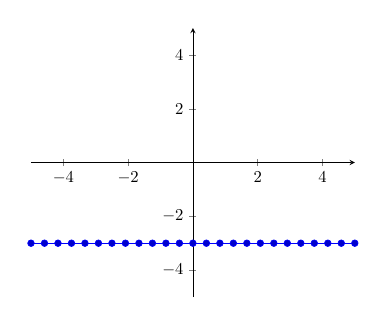
\begin{tikzpicture}[scale=0.6]
        \begin{axis}[xmin=-5, xmax=5, ymin=-5, ymax=5, axis lines=middle]
            \addplot{-3};
        \end{axis}
        \end{tikzpicture}
        \caption{$f(x) = -3$}
        \end{figure}

        \skipframe

        \item $D(f) = \R$ e $Im(f) = [0, \infty)$

        \begin{figure}
        \centering
        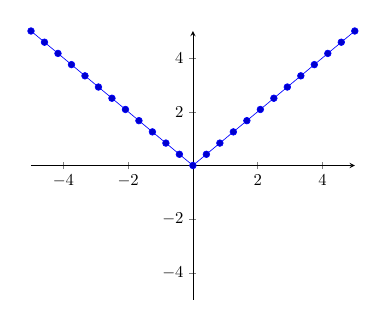
\begin{tikzpicture}[scale=0.6]
        \begin{axis}[xmin=-5, xmax=5, ymin=-5, ymax=5, axis lines=middle]
            \addplot{abs(x)};
        \end{axis}
        \end{tikzpicture}
        \caption{$f(x) = \abs{x}$}
        \end{figure}

        \item <colocar gráficos>

        \skipframe

        \item $D(f) = [-2, 6)$ e $Im(f) = [-2, 4]$

        \item $D(f) = [3, \infty) - {5}$

        \item $(1/2, \infty)$

        \skipframe

        \item $D(f) = (-\infty, \infty) - {5}$ e $Im(f) = [-1, \infty)$. O gráfico de $f$ corresponde ao do valor absoluto deslocado duas unidades para a direita e uma unidade verticalmente.

        \vspace{0.5cm}

        \begin{figure}
        \centering
        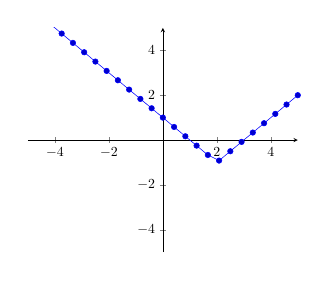
\begin{tikzpicture}[scale=0.5]
        \begin{axis}[xmin=-5, xmax=5, ymin=-5, ymax=5, axis lines=middle]
            \addplot{abs(x-2)-1};
        \end{axis}
        \end{tikzpicture}
        \caption{$f(x) = \abs{x-2}-1$}
        \end{figure}

        \skipframe

        \item 
        \begin{enumerate}[a]
            \item Posição 4.
            \item Posição 1.
            \item Posição 2.
            \item Posição 3.
        \end{enumerate}
    \end{enumerate}
\end{frame}